\documentclass[11pt,preprint, authoryear]{elsarticle}

\usepackage{lmodern}
%%%% My spacing
\usepackage{setspace}
\setstretch{1.2}
\DeclareMathSizes{12}{14}{10}{10}

% Wrap around which gives all figures included the [H] command, or places it "here". This can be tedious to code in Rmarkdown.
\usepackage{float}
\let\origfigure\figure
\let\endorigfigure\endfigure
\renewenvironment{figure}[1][2] {
    \expandafter\origfigure\expandafter[H]
} {
    \endorigfigure
}

\let\origtable\table
\let\endorigtable\endtable
\renewenvironment{table}[1][2] {
    \expandafter\origtable\expandafter[H]
} {
    \endorigtable
}


\usepackage{ifxetex,ifluatex}
\usepackage{fixltx2e} % provides \textsubscript
\ifnum 0\ifxetex 1\fi\ifluatex 1\fi=0 % if pdftex
  \usepackage[T1]{fontenc}
  \usepackage[utf8]{inputenc}
\else % if luatex or xelatex
  \ifxetex
    \usepackage{mathspec}
    \usepackage{xltxtra,xunicode}
  \else
    \usepackage{fontspec}
  \fi
  \defaultfontfeatures{Mapping=tex-text,Scale=MatchLowercase}
  \newcommand{\euro}{€}
\fi

\usepackage{amssymb, amsmath, amsthm, amsfonts}

\def\bibsection{\section*{References}} %%% Make "References" appear before bibliography


\usepackage[round]{natbib}

\usepackage{longtable}
\usepackage[margin=2.3cm,bottom=2cm,top=2.5cm, includefoot]{geometry}
\usepackage{fancyhdr}
\usepackage[bottom, hang, flushmargin]{footmisc}
\usepackage{graphicx}
\numberwithin{equation}{section}
\numberwithin{figure}{section}
\numberwithin{table}{section}
\setlength{\parindent}{0cm}
\setlength{\parskip}{1.3ex plus 0.5ex minus 0.3ex}
\usepackage{textcomp}
\renewcommand{\headrulewidth}{0.2pt}
\renewcommand{\footrulewidth}{0.3pt}

\usepackage{array}
\newcolumntype{x}[1]{>{\centering\arraybackslash\hspace{0pt}}p{#1}}

%%%%  Remove the "preprint submitted to" part. Don't worry about this either, it just looks better without it:
\makeatletter
\def\ps@pprintTitle{%
  \let\@oddhead\@empty
  \let\@evenhead\@empty
  \let\@oddfoot\@empty
  \let\@evenfoot\@oddfoot
}
\makeatother

 \def\tightlist{} % This allows for subbullets!

\usepackage{hyperref}
\hypersetup{breaklinks=true,
            bookmarks=true,
            colorlinks=true,
            citecolor=blue,
            urlcolor=blue,
            linkcolor=blue,
            pdfborder={0 0 0}}


% The following packages allow huxtable to work:
\usepackage{siunitx}
\usepackage{multirow}
\usepackage{hhline}
\usepackage{calc}
\usepackage{tabularx}
\usepackage{booktabs}
\usepackage{caption}


\newenvironment{columns}[1][]{}{}

\newenvironment{column}[1]{\begin{minipage}{#1}\ignorespaces}{%
\end{minipage}
\ifhmode\unskip\fi
\aftergroup\useignorespacesandallpars}

\def\useignorespacesandallpars#1\ignorespaces\fi{%
#1\fi\ignorespacesandallpars}

\makeatletter
\def\ignorespacesandallpars{%
  \@ifnextchar\par
    {\expandafter\ignorespacesandallpars\@gobble}%
    {}%
}
\makeatother

\newenvironment{CSLReferences}[2]{%
}

\urlstyle{same}  % don't use monospace font for urls
\setlength{\parindent}{0pt}
\setlength{\parskip}{6pt plus 2pt minus 1pt}
\setlength{\emergencystretch}{3em}  % prevent overfull lines
\setcounter{secnumdepth}{5}

%%% Use protect on footnotes to avoid problems with footnotes in titles
\let\rmarkdownfootnote\footnote%
\def\footnote{\protect\rmarkdownfootnote}
\IfFileExists{upquote.sty}{\usepackage{upquote}}{}

%%% Include extra packages specified by user

%%% Hard setting column skips for reports - this ensures greater consistency and control over the length settings in the document.
%% page layout
%% paragraphs
\setlength{\baselineskip}{12pt plus 0pt minus 0pt}
\setlength{\parskip}{12pt plus 0pt minus 0pt}
\setlength{\parindent}{0pt plus 0pt minus 0pt}
%% floats
\setlength{\floatsep}{12pt plus 0 pt minus 0pt}
\setlength{\textfloatsep}{20pt plus 0pt minus 0pt}
\setlength{\intextsep}{14pt plus 0pt minus 0pt}
\setlength{\dbltextfloatsep}{20pt plus 0pt minus 0pt}
\setlength{\dblfloatsep}{14pt plus 0pt minus 0pt}
%% maths
\setlength{\abovedisplayskip}{12pt plus 0pt minus 0pt}
\setlength{\belowdisplayskip}{12pt plus 0pt minus 0pt}
%% lists
\setlength{\topsep}{10pt plus 0pt minus 0pt}
\setlength{\partopsep}{3pt plus 0pt minus 0pt}
\setlength{\itemsep}{5pt plus 0pt minus 0pt}
\setlength{\labelsep}{8mm plus 0mm minus 0mm}
\setlength{\parsep}{\the\parskip}
\setlength{\listparindent}{\the\parindent}
%% verbatim
\setlength{\fboxsep}{5pt plus 0pt minus 0pt}



\begin{document}



\begin{frontmatter}  %

\title{Music Taste Across Time}

% Set to FALSE if wanting to remove title (for submission)




\author[Add1]{Anna Mayer}
\ead{28776534@sun.ac.za}





\address[Add1]{Stellenbosch University}


\begin{abstract}
\small{
This report analyses the longevity and musical progression of some of
the most famous bands over time, focussing specifically on a comparison
of Metallica and Coldplay. While Coldplay is a relatively young band
compared to Metallica, both have been sucessful and very popular as one
can see in the graphs of this report.
}
\end{abstract}

\vspace{1cm}


\begin{keyword}
\footnotesize{
Spotify \sep Coldplay \sep Metallica \\
\vspace{0.3cm}
}
\end{keyword}



\vspace{0.5cm}

\end{frontmatter}

\setcounter{footnote}{0}



%________________________
% Header and Footers
%%%%%%%%%%%%%%%%%%%%%%%%%%%%%%%%%
\pagestyle{fancy}
\chead{}
\rhead{}
\lfoot{}
\rfoot{\footnotesize Page \thepage}
\lhead{}
%\rfoot{\footnotesize Page \thepage } % "e.g. Page 2"
\cfoot{}

%\setlength\headheight{30pt}
%%%%%%%%%%%%%%%%%%%%%%%%%%%%%%%%%
%________________________

\headsep 35pt % So that header does not go over title




\hypertarget{introduction}{%
\section{\texorpdfstring{Introduction
\label{Introduction}}{Introduction }}\label{introduction}}

This report analyses the longevity and musical progression of some of
the most famous bands over time. It looks into different data sets
provided on popularity and other interesting determinants of music like
valence of songs. The main focus lies on the musical progression of the
two bands over time and their popularity in general.

\hypertarget{data}{%
\section{Data}\label{data}}

The data used for analysis focuses on the two bands Metallica and
Coldplay. Moreover, data from Spotify and the Billboard Top 100 list
were used for the analysis below.

\hypertarget{analysis}{%
\section{Analysis}\label{analysis}}

Let us first have a closer look at the popularity by album for each of
the bands individually:

\begin{figure}[H]

{\centering \includegraphics{Question2_files/figure-latex/Figure1-1} 

}

\caption{Popularity by album of Metallica \label{Figure1}}\label{fig:Figure1}
\end{figure}

As one can see, there is large variation in the popularity by album for
Metallica. The on average most succesful album seems to be 72 Seasons.
The on average least successful album seems to be Master of Puppets
(Deluxe Box Set/ Remastered).

In a next step, let us have a closer look at Coldplay:

\begin{figure}[H]

{\centering 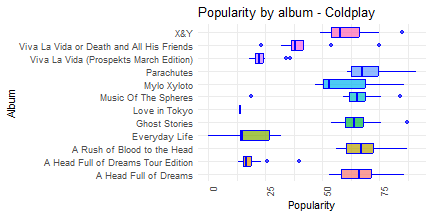
\includegraphics{Question2_files/figure-latex/Figure2-1} 

}

\caption{Popularity by album for Coldplay \label{Figure2}}\label{fig:Figure2}
\end{figure}

Again, we can see that some albums are more popular than others.
Parachutes seems to be the most popular ablum whereas, Love in Tokyo and
Everyday Life do not seem to be comparatively very popular.

Let us now compare the two bands and their popularity over time:

\begin{figure}[H]

{\centering \includegraphics{Question2_files/figure-latex/Figure3-1} 

}

\caption{Average Popularity Scores over Time \label{Figure3}}\label{fig:Figure3}
\end{figure}

As one can see in the graph above, Coldplay only exists since 1997.
However, their popularity was directly relatively high from the
beginning. Using the release date of the different albums to refer to
the years the bands were active, one can see, that there is in the
beginning for Metallica a large variation across albums. For Coldplay,
when they started releasing around 2000, their first albums were
directly a huge success. However, variation of the popularity for the
Coldplay albums increased overt time. In general, the popularity score
ranges from 0 to 100. One might wonder what the popularity score
actually consists of and which criteria are used to assign points. If
one wants to dig deeper into the sphere of popularity scores, Koutlis,
Schinas, Papadopoulos \& Kompatsiaris
(\protect\hyperlink{ref-info11060323}{2020}) provide a novel approach to
assigning popularity scores.

Another interesting aspect for comparison could be how often the two
bands Coldplay and Metallica were in the top 100 Billboard charts:

\begin{figure}[H]

{\centering 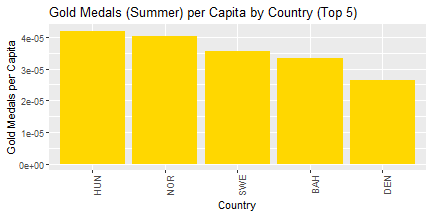
\includegraphics{Question2_files/figure-latex/Figure4-1} 

}

\caption{Amount of top 10 in Billboard 100 (no features) \label{Figure4}}\label{fig:Figure4}
\end{figure}

Note that featurings are not included in the count. This graph is
comparing Coldplay and Metallica with the singer/band that was ranked
most in the top 10 of the Billboard top 100 ranking over time. Mariah
Carey is clearly the winner here. Nevertheless, Coldplay was 19 times in
the top 10 and Metallica once.

Comparing it to the total amount of times the two bands appeared in the
top 100, Coldplay was ranked there 281 times and Metallica 197, which is
remarkable, as Coldplay only exists since 1997 and Metallica longer.
However, he different genres and the fact that Metallica probably
adresses a smaller group of listeners, might explain that difference.

Finally, comparing and analyzing how valence developed over time for
Metallica and Coldplay Valence ``describes the musical positiveness
conveyed by a track. Tracks with high valence sound more positive
(e.g.~happy, cheerful, euphoric), while tracks with low valence sound
more negative (e.g.~sad, depressed, angry)''.

\begin{figure}[H]

{\centering 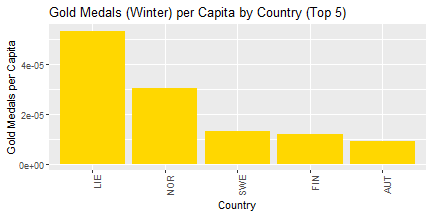
\includegraphics{Question2_files/figure-latex/Figure5-1} 

}

\caption{Valence over time \label{Figure5}}\label{fig:Figure5}
\end{figure}

As one can see, there is a large variation in average valence,
especially for Coldplay. However, for Metallica there seems to be a
downward trend since the end of the 1990s, meaning that tracks of
Metallica seem to sound more negative on average recently. For Coldplay,
it varies a lot, even more than Metallica, which might be a reason for
their success as they address both groups, those that prefer more
negative and those that prefer more positive music. In the 2010s the
music seems however also to be more negative for Coldplay.

\hypertarget{conclusion}{%
\section{Conclusion}\label{conclusion}}

To conclude, one can say, that both bands are clearly popular and
famous. Some albums are more popular than others and although Coldplay
is younger, they have more top 10 rankings and also in general top 100
rankings in the billboard ranking than Metallica. One reason might be
that Coldplay maybe addresses a larger amount of listeners given that
they cover a larger spectrum of for example valence in their music but
also address listeners of a genre in general that is probably more
popular than the genre Metallica is in.

\newpage

\hypertarget{references}{%
\section*{References}\label{references}}
\addcontentsline{toc}{section}{References}

\hypertarget{refs}{}
\begin{CSLReferences}{1}{0}
\leavevmode\vadjust pre{\hypertarget{ref-info11060323}{}}%
Koutlis, C., Schinas, M., Papadopoulos, S. \& Kompatsiaris, I. 2020.
\href{https://doi.org/10.3390/info11060323}{GAP: Geometric aggregation
of popularity metrics}. \emph{Information}. 11(6).

\end{CSLReferences}

\bibliography{Tex/ref}





\end{document}
